% Karrera Amarierako Proiektua egiteko LaTeX txantiloia
% itsas.ehu.es/workgroups/latex
% Unai Martinez Corral
% umartinez012@ikasle.ehu.es
%
% <- sectb_main.tex

\titlesubsection{Co-simulation}

\begin{table}[!htp]
\centering
\begin{tabular}[c]{c||c|c|c}
 & & & \\
 & {\Large$Kp$} & {\Large$Ki$} & {\Large$Kd$} \\
 & & & \\
\hline
\hline
 & & & \\
\textbf{Hamartarra} & $6$ & $6,875\cdot 10^{-4}$ & $22,7272$ \\
\small{Zehatza} & & & \\
 & & & \\
\textbf{7 bit} & 0000110. & {\tiny[0.0000000000]}1011011 & 10110.11 \\
 & & & \\
\textbf{Zeinua} & 00000110 & 01011011 & 01011011 \\
\small{8 bit} & & & \\
 & & & \\
\textbf{Hamartarra} & $6$ & $6,943 \cdot 10^{-4}$ & $22.75$ \\
\small{8 bitetik} &
 \multirow{2}{*}{\footnotesize $\begin{matrix}\Delta0\\\%0\end{matrix}$} &
 \multirow{2}{*}{\footnotesize $\begin{matrix}\Delta6,8\cdot 10^{-6}\\\%0,9891\end{matrix}$} &
 \multirow{2}{*}{\footnotesize $\begin{matrix}\Delta0,0228\\\%0,1\end{matrix}$} \\
\small{bihurtuta} & & & \\
 & & & \\
\textbf{Formatoa} & Fix\_8\_0 & Fix\_8\_17 & Fix\_8\_2 \\
 & & & \\
\end{tabular}
\caption[Konstanteei esleitu beharreko hitz bitarrak kalkulatzea]{Balio zehatzetatik abiatuta, konstanteen seinaleei esleitu beharreko hitz bitarren kalkulua.}
\label{tab:vhdl_coef}
\end{table}

Blokearen konfigurazio aukeretan \emph{Simulation mode} aukeran \emph{ISE Simulator} aukeratuko dugu. Honela egingo ez bagenu, \emph{Simulink}ek beste blokea guztien kalkuluak burutuko lituzke, baina \emph{Blackbox}eko irteera guztien balioa zero izango litzateke.

Zuzenean simulazioa eginez gero, grafikoetan antzemango dugu irteerak balio oso altuak dituela, eta kontrola ezinezkoa dela. Gure VHDL kontroladorearen irteeraren koma bitarra, aurreko atalean adierazi bezala, ez dago $lsb$an ezta $minbp$ parametroak adierazitakoan. \emph{Simulink}ek ez du sarreren koma bitarraren kokapena kontuan hartzen eta ondorioz interpretatzean $2^8$ aldiz biderkatzen du irteeraren balioa.

\begin{figure}[!htp]
\centering
% Karrera Amarierako Proiektua egiteko LaTeX txantiloia
% itsas.ehu.es/workgroups/latex
% Unai Martinez Corral
% umartinez012@ikasle.ehu.es
%
% <- sectb_last.tex

\tikzstyle{inout} = [rectangle]
\tikzstyle{gate} = [draw, rectangle, fill=orange!25, minimum height=3ex,minimum width=4.5em]
\tikzstyle{mem} = [draw, rectangle, minimum height=3ex,minimum width=4.5em]
\tikzstyle{block} = [draw, rectangle, fill=green!25, minimum height=13em, minimum width=4.5em]

\tikzstyle{mgate} = [draw, circle, fill=orange!25,minimum width=1em]
\tikzstyle{mmem} = [draw, circle,minimum width=1em]
\tikzstyle{mblock} = [draw, circle, fill=green!25, minimum width=1em]

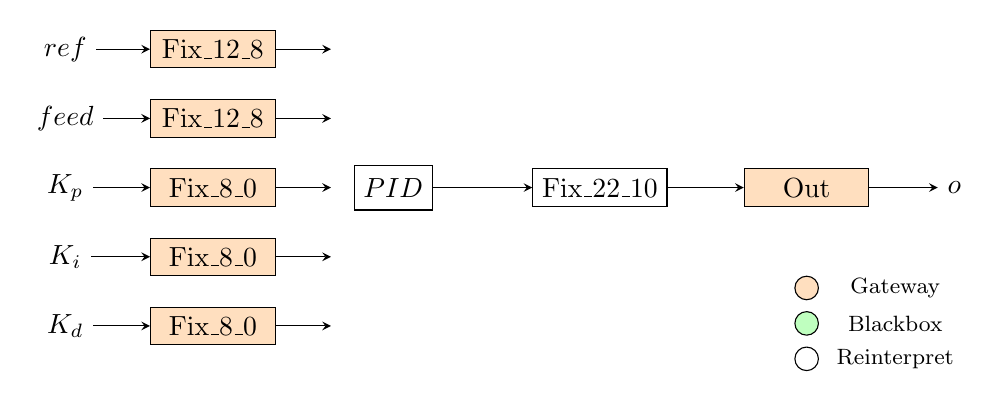
\begin{tikzpicture}[auto, node distance=.75cm,>=stealth]
  \def\sep{1.5cm}
  \def\bh{2.5em}
  \def\bw{2.25em}

  \node[block](pid){$PID$};
  \node [coordinate, left of=pid,node distance=\bw](kp_p){};
  \node [coordinate, above of=kp_p,node distance=\bh](f_p){};
  \node [coordinate, above of=f_p,node distance=\bh](r_p){};
  \node [coordinate, below of=kp_p,node distance=\bh](ki_p){};
  \node [coordinate, below of=ki_p,node distance=\bh](kd_p){};

  \node [gate, left of=r_p,node distance=\sep] (r_g) {Fix\_12\_8};
  \node [gate, left of=f_p,node distance=\sep] (f_g) {Fix\_12\_8};
  \node [gate, left of=kp_p,node distance=\sep] (kp_g) {Fix\_8\_0};
  \node [gate, left of=ki_p,node distance=\sep] (ki_g) {Fix\_8\_0};
  \node [gate, left of=kd_p,node distance=\sep] (kd_g) {Fix\_8\_0};

  \node [inout, left of=r_g, node distance=1.25*\sep] (r) {$ref$};
  \node [inout, left of=f_g, node distance=1.25*\sep] (f) {$feed$};
  \node [inout, left of=kp_g, node distance=1.25*\sep] (kp) {$K_p$};
  \node [inout, left of=ki_g, node distance=1.25*\sep] (ki) {$K_i$};
  \node [inout, left of=kd_g, node distance=1.25*\sep] (kd) {$K_d$};

  \node [mem, right of=pid,node distance=1.75*\sep] (reint) {Fix\_22\_10};
  \node [gate, right of=reint,node distance=1.75*\sep] (gate_out) {Out};
  \node [inout, right of=gate_out,node distance=1.25*\sep] (o) {$o$};
   
\footnotesize

  \node [mgate, below of=gate_out, node distance=.85*\sep] (lgate) {};
  \node [inout, right of=lgate,node distance=.75*\sep] (ltgate) {Gateway};
  \node [mblock, below of=lgate,node distance=.3*\sep] (lblock) {};
  \node [inout, right of=lblock,node distance=.75*\sep] (ltblock) {Blackbox};
  \node [mmem, below of=lblock,node distance=.3*\sep] (lmem) {};
  \node [inout, right of=lmem,node distance=.75*\sep] (ltmem) {Reinterpret};
  
  \draw [->]  (r_g) -- (r_p);
  \draw [->] (f_g) -- (f_p);
  \draw [->] (kp_g) -- (kp_p);
  \draw [->] (ki_g) -- (ki_p);
  \draw [->] (kd_g) -- (kd_p);

  \draw [->]  (r) -- (r_g);
  \draw [->] (f) -- (f_g);
  \draw [->] (kp) -- (kp_g);
  \draw [->] (ki) -- (ki_g);
  \draw [->] (kd) -- (kd_g);

  \draw [->] (pid) -- (reint);
  \draw [->] (reint) -- (gate_out);
  \draw [->] (gate_out) -- (o);
  
\end{tikzpicture}

\caption[Modeloa: \emph{Blackbox} (kontroladorea)]{\emph{Blackbox} blokea erabiltzeko kontroladorearen modeloa ($K_p=24$ eta $K_i=K_d=91$).}
\label{fig:mod_box}
\end{figure}

Nahiz eta hitz tamaina mugatu, parametroekin adierazpenak aldatu eta eskuz egindako VHDL deskribapena erabilita, azkeneko modelo honek modelo jarraituarekiko duen ezberdintasuna funtsean diskretu izateagatik dela iritzi dezakegu, guk egindako pausu guztiek eragindako erroreak oso txikitzat hartuz ($\%0,5$-tik behera).

\begin{figure}[!htp]
\centering
%Anie - ohkis.sourceforge.net
%Unai Martinez Corral
%umartinez012@ikasle.ehu.es
%
% <- ./cases/anie_s3etiny_man.tex

\tikzstyle{inout} = [rectangle]
\tikzstyle{block} = [draw, rectangle, minimum height=1.625em, minimum width=2em]
\tikzstyle{lblock} = [draw, rectangle, minimum height=1.5em, minimum width=1.5em]
\tikzstyle{cblock} = [draw, rectangle, minimum height=1.625em, minimum width=2.25em]
\tikzstyle{reg} = [draw,rectangle, minimum height=5em, minimum width=4em]
\tikzstyle{co} = [draw, rectangle, minimum height=9em, minimum width=18em]
\tikzstyle{count} = [draw,fill=black!15,rectangle, minimum height=7.5em, minimum width=10.5em]

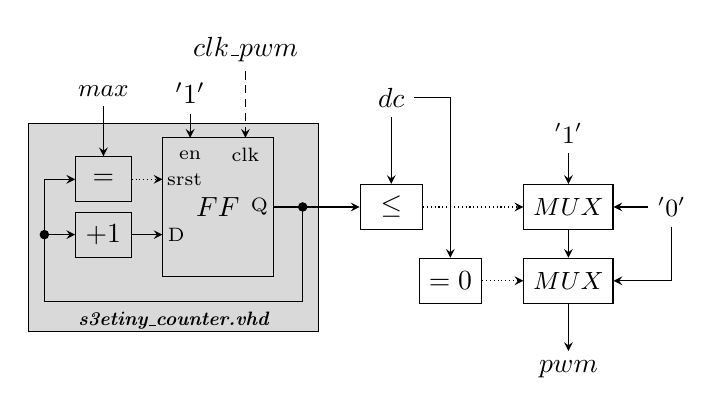
\begin{tikzpicture}[auto, node distance=2cm,>=stealth]
  \def\sep{1.5cm}
  \def\sepl{.25em}
  \def\bh{5em}
  \def\bhb{.3em}
 \def\bw{4em}
  \def\bwb{1em}

%% H
 
  \node[count](ffall){};
  \node[inout,below of=ffall,node distance=3.375em](lg){\scriptsize\bfseries\itshape s3etiny\_counter.vhd};

  \node[coordinate,above of=ffall, node distance=3*\sepl](ffp){};
  \node[reg,right of=ffp, node distance=.375*\sep](ff){$FF$};

  \node[coordinate,right of=ff,node distance=.5*\bw](ffe){};
  \node[coordinate,above of=ffe,node distance=.3*\bh](ffea){};
  \node[coordinate, left of=ff,node distance=.5*\bw](ffw){};
  \node[coordinate,above of=ffw,node distance=.2*\bh](ffwa){};
  \node[coordinate,left of=ffwa,node distance=2*\sepl](ffwa_l){};
  \node[coordinate,below of=ffw,node distance=.2*\bh](ffwb){};
  \node[block,left of=ffwa,node distance=.5*\sep](comp){$=$};
  \node[block,left of=ffwb,node distance=.5*\sep](countn){$+1$};
  \node[coordinate,left of=countn,node distance=.5*\sep](countn_w){};

  \node[coordinate,above of=ff,node distance=.5*\bh](ffa){};
  \node[coordinate,left of=ffa,node distance=.25*\bw](ffaw){};
  \node[coordinate,right of=ffa,node distance=.25*\bw](ffae){};

  \node[inout,below of=ffaw,node distance=.125*\bh](e){\scriptsize en};
  \node[inout,below of=ffae,node distance=.125*\bh](c){\scriptsize clk};
  \node[inout,right of=ffwa,node distance=.2*\bw](srst){\scriptsize srst};
  \node[inout,right of=ffwb,node distance=.125*\bw](d){\scriptsize D};
  \node[inout,left of=ffe,node distance=.125*\bw](d){\scriptsize Q};

  \node[inout,above of=comp,node distance=.75*\sep](limit){\small $max$};

  \node[coordinate,right of=ffe,node distance=.25*\sep](un){};
  \node[coordinate,below of=un,node distance=.625*\sep](un_b){};
  \node[coordinate,below of=un_b,node distance=3*\sepl](un_bb){};

  \node[cblock, right of=un, node distance=.75*\sep](dcc){$\leq$};
  \node[cblock, right of=un_b, node distance=1.25*\sep](zero){$=0$};

  \node[block,right of=dcc,node distance=1.5*\sep](mux){\small $MUX$};
  \node[inout,right of=mux,node distance=.875*\sep](mux0){\small $'0'$};
  \node[inout,above of=mux,node distance=.625*\sep](mux1){\small $'1'$};

  \node[block,right of=zero,node distance=1*\sep](omux){\small $MUX$};
  \node[coordinate,right of= omux,node distance=.625*\sep](omux_r){};
  \node[inout,below of=omux,node distance=.75*\sep](pwm){$pwm$};

  \node[coordinate,above of=ffae,node distance=.625*\sep](ffae_a){};
  \node[coordinate,above of=ffaw,node distance=.625*\sep](en){};

  \node[inout,above of=ffaw,node distance=.375*\sep](en){$'1'$};
  \node[inout,above of=ffae,node distance=.75*\sep](clk){$clk\_pwm$};
  \node[inout,above of=dcc,node distance=.75*\sep+.75em](dc){$dc$};

  \draw[fill](un) circle (1.5pt);
  \draw[fill](countn_w) circle (1.5pt);

  \draw[->](limit) -- (comp);
  \draw[->,densely dotted](comp) -- (ffwa);
  \draw[->](countn) -- (ffwb);
  \draw[->](un) -- (un_b) -- (un_bb) -| (countn_w) -- (countn);
  \draw[->](countn_w) |- (comp);
  \draw[->](en) -- (ffaw);
  \draw[->,densely dashed](clk) -- (ffae);
  
  \draw[->](ffe) -- (dcc);
  \draw[->](dc) -| (zero);

  \draw[->](dc) -- (dcc);
  \draw[->](mux) -- (omux);
  \draw[->,densely dotted](dcc) -- (mux);
  \draw[->](mux0) -- (mux);
  \draw[->](mux1) -- (mux);
  \draw[->](mux0) |- (omux);
  \draw[->,densely dotted](zero) -- (omux);
  \draw[->](omux) -- (pwm);

\end{tikzpicture}

\caption{PWM seinalea sortzea.}
\label{fig:pwm}
\end{figure}

\begin{figure}[!htp]
\centering
%Anie - ohkis.sourceforge.net
%Unai Martinez Corral
%umartinez012@ikasle.ehu.es
%
% <- ./cases/anie_s3etiny_man.tex

\usetikzlibrary{shapes,arrows}

\tikzstyle{decision} = [diamond, draw, text width=4.5em, text badly centered, inner sep=0pt]
\tikzstyle{state} = [rectangle, draw, fill=black!15, text width=5.25em, text centered, minimum height=3.5em]
\tikzstyle{action} = [draw, ellipse]

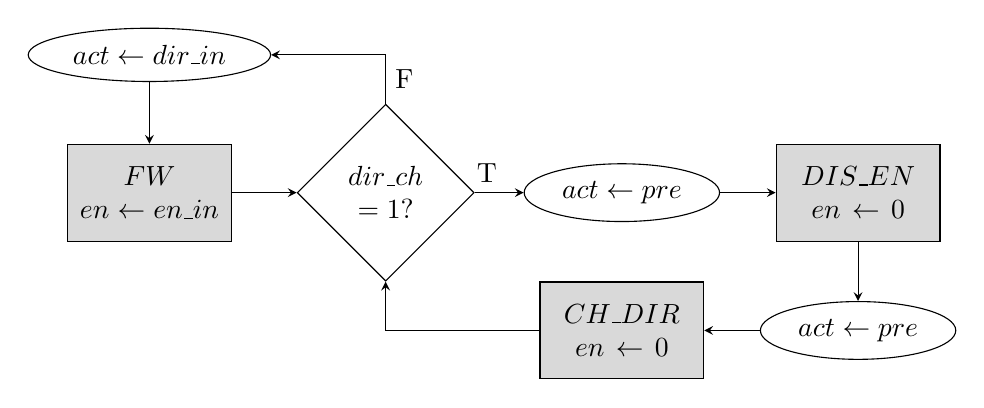
\begin{tikzpicture}[auto, node distance=3cm,>=stealth]
\def\sep{3.5cm} 

  \node[state](fw){$FW$\\$en \leftarrow en\_in$};
  \node[decision,right of=fw](fwd){$dir\_ch$\\$=1?$};
  \node[action,above of=fw,node distance=.5*\sep](fwb){$act \leftarrow dir\_in$};
  \node[action,right of=fwd](fwc){$act \leftarrow pre$};

  \node[state,right of=fwc](dis_en){$DIS\_EN$\\$en \leftarrow 0$};
  \node[action,below of=dis_en,node distance=.5*\sep](dis_ena){$act \leftarrow pre$};

  \node[state,left of=dis_ena](ch_dir){$CH\_DIR$\\$en \leftarrow 0$};

  \draw[->](fw) -- (fwd);
  \draw[->](fwd) |- node [near start,right] {F} (fwb);
  \draw[->](fwb) -- (fw);
  \draw[->](fwd) -- node [near start] {T} (fwc);
  \draw[->](fwc) -- (dis_en);
  \draw[->](dis_en) -- (dis_ena);
  \draw[->](dis_ena) -- (ch_dir);
  \draw[->](ch_dir) -| (fwd);
%  \draw[->](ch_dir) -- (ch_dira);
 % \draw[->](ch_dira) -- (ch_dird);
 % \draw[->](ch_dird) -- node [near start,above] {F} (ch_dirb);
 % \draw[->](ch_dird) -- node [near start] {T} (ch_dirc);
 % \draw[->](ch_dirc) -- (ch_dir);

%  \node[count](ffall){};
%  \node[decision,below of=ffall](dec){};
%  \node[state,below of=dec](st){};
 % \node[action,below of=st](act){};
 % \node[cloud,below of=act](cl){$dir\_out \leftarrow dir\_pre$};

\end{tikzpicture}

\caption{FSM adibidea.}
\label{fig:hbridge}
\end{figure}